%\renewcommand{\theequation}{\theenumi}
%\begin{enumerate}[label=\arabic*.,ref=\thesubsection.\theenumi]
%\numberwithin{equation}{enumi}
    \item Solve $30x < 200$ when
    \begin{enumerate} 
    \item  x is a natural number,
    \item x is an integer.
\end{enumerate}
\solution From the given information, 
\begin{align}
30x < 200 \implies x < \frac{20}{3}
\label{eq:lineq_nat}
\end{align}
If $x$ is a natural number, $x \in \cbrak{1, 2, 3, 4, 5, 6}$. If $x$ is an integer, then the solution set includes 0 as well as all negative integers.
    \item Solve $5x-3 < 3x+1$ when
    \begin{enumerate} 
\item  x is an integer,
    \item x is a real number.
\end{enumerate}
\solution 
\begin{align}
5x-3 < 3x+1 \implies x < 2
\label{eq:lineq_real}
\end{align}
%
If $x$ is real, then $x \in \brak{-\infty, 2}$. 
%Fig.  provides a graphical solution using the following python code
%\begin{lstlisting}
%\end{lstlisting}
    \item Solve the following system of linear inequalities graphically.
\begin{align}
\label{eq:line_two_ineq}
\begin{split}
    x+y &\geq 5
\\
    x-y &\leq 3
\end{split}
\end{align}
\solution  Let $u_1 \ge 0, u_2 \ge 0$.  This may be expressed as
\begin{align}
\vec{u} = \myvec{u_1\\u_2}\succeq \vec{0}
\end{align}
%
\eqref{eq:line_two_ineq} can then be expressed as
\begin{align}
\begin{split}
    x+y &\geq 5
\\
    -x+y &\geq -3
\end{split}
%
\\
\implies 
\myvec{1 & 1 \\ -1 & 1}\vec{x}  &\succeq \myvec{5\\-3}
\\
\myvec{1 & 1 \\ -1 & 1}\vec{x}  -\vec{u}&=\myvec{5\\-3}
\\
\text{or, }
\myvec{1 & 1 \\ -1 & 1}\vec{x} &= \myvec{5\\-3} +\vec{u}
\end{align}
%
resulting in 
\begin{align}
\vec{x} &= \myvec{1 & 1 \\ -1 & 1}^{-1}\myvec{5\\-3} +\myvec{1 & 1 \\ -1 & 1}^{-1}\vec{u}
\\
\text{or, } \vec{x} &= \myvec{4\\1} +\frac{1}{2}\myvec{1 & -1 \\ 1 & 1}\vec{u}
\end{align}
%
after obtaining the  inverse.
%
 Fig. \ref{fig:line_ineq} generated using the following python code shows the region satisfying \eqref{eq:line_two_ineq}

\begin{lstlisting}
codes/line/line_ineq.py
\end{lstlisting}
%
\begin{figure}[!ht]
\includegraphics[width=\columnwidth]{./line/figs/line_ineq.eps}
\caption{}
\label{fig:line_ineq}
\end{figure}
%
\item Solve 
\begin{align}
\begin{split}
2x+y \geq 4
\\ 
x+y \leq 3
\\ 
2x-3y \leq 6
\end{split}
\label{eq:line_mult_ineq}
\end{align}
%
\\
\solution  Fig. \ref{fig:line_ineq_mult} generated using the following python code shows the region satisfying \eqref{eq:line_mult_ineq}

\begin{lstlisting}
codes/line/line_ineq_mult.py
\end{lstlisting}
%
\begin{figure}[!ht]
\includegraphics[width=\columnwidth]{./line/figs/line_ineq_mult.eps}
\caption{}
\label{fig:line_ineq_mult}
\end{figure}
%
\item   Solve    $x+y < 5$ graphically.
\\
\solution 
\input{./solutions/5/chapters/lines/docq6.tex}
%
    \item Solve 
\begin{align}
\myvec{3 & 2 \\ 1 & 4 \\ 1 & 0 \\ 0 & -1 \\ -1 & 0} \vec{x}\preceq \myvec{150\\80\\15\\0\\0}
%3x+2y \leq 150
%\\ 
%x+4y \leq 80
%\\ 
%x \leq 15
%\\ 
%y \geq 0
%\\
%x \geq 0 
\end{align}
%
   
%    \end{enumerate}
\item Solve  x $\geq$ 3, y $\geq$ 2 graphically.
\\
\solution 
%
\begin{align}
    E(X) &= \frac{1}{\sqrt{2\pi}} \int_{-\infty}^{\infty} x e^{-\frac{x^2}{2}}dx\\
    &=0 \quad \brak{ \text{ odd function}}
\end{align}
\begin{align}
    E\brak{X^2}&= \frac{1}{\sqrt{2\pi}}\int_{-\infty}^{\infty} x^2
e^ {-\frac{x^2}{2}} dx \quad \brak{even function}\\
    &= \frac{2}{\sqrt{2\pi}} \int_{0}^{\infty} x^2 e^{-\frac{x^2}{2}} dx\\
    &= \frac{2}{\sqrt{2\pi}}\int_{0}^{\infty}\sqrt{2u}e^{-u} du \quad\brak{Let \frac{x^2}{2}= u}\\
    &= \frac{2}{\sqrt{\pi}} \int_{0}^{\infty} e^{-u} u^{\frac{3}{2}-1} du\\
    &= \frac{2}{\sqrt{\pi}} \Gamma\brak{{\frac{3}{2}}}\\
    &= \frac{1}{\sqrt{\pi}}\Gamma\brak{\frac{1}{2}} \\
    &= 1
\end{align}
where we have used the fact that
\begin{align}
\quad\because \Gamma(n)= (n-1)\Gamma(n-1); \Gamma\brak{\frac{1}{2}}=\sqrt{\pi}
\end{align}
%
Thus, the  variance is
\begin{align}
    \sigma^2 =  E\brak X^2 - E^2\brak X = 1
\end{align}


    \item Solve 7x+3 $<$ 5x+9. Show the graph of the solutions on number line.
\\
\solution 
%
\begin{align}
    E(X) &= \frac{1}{\sqrt{2\pi}} \int_{-\infty}^{\infty} x e^{-\frac{x^2}{2}}dx\\
    &=0 \quad \brak{ \text{ odd function}}
\end{align}
\begin{align}
    E\brak{X^2}&= \frac{1}{\sqrt{2\pi}}\int_{-\infty}^{\infty} x^2
e^ {-\frac{x^2}{2}} dx \quad \brak{even function}\\
    &= \frac{2}{\sqrt{2\pi}} \int_{0}^{\infty} x^2 e^{-\frac{x^2}{2}} dx\\
    &= \frac{2}{\sqrt{2\pi}}\int_{0}^{\infty}\sqrt{2u}e^{-u} du \quad\brak{Let \frac{x^2}{2}= u}\\
    &= \frac{2}{\sqrt{\pi}} \int_{0}^{\infty} e^{-u} u^{\frac{3}{2}-1} du\\
    &= \frac{2}{\sqrt{\pi}} \Gamma\brak{{\frac{3}{2}}}\\
    &= \frac{1}{\sqrt{\pi}}\Gamma\brak{\frac{1}{2}} \\
    &= 1
\end{align}
where we have used the fact that
\begin{align}
\quad\because \Gamma(n)= (n-1)\Gamma(n-1); \Gamma\brak{\frac{1}{2}}=\sqrt{\pi}
\end{align}
%
Thus, the  variance is
\begin{align}
    \sigma^2 =  E\brak X^2 - E^2\brak X = 1
\end{align}

    \item Solve $\frac{3x-4}{2} \geq \frac{x+1}{4}-1$. Show the graph of the solutions on number line.
\\
\solution 
%
\begin{align}
    E(X) &= \frac{1}{\sqrt{2\pi}} \int_{-\infty}^{\infty} x e^{-\frac{x^2}{2}}dx\\
    &=0 \quad \brak{ \text{ odd function}}
\end{align}
\begin{align}
    E\brak{X^2}&= \frac{1}{\sqrt{2\pi}}\int_{-\infty}^{\infty} x^2
e^ {-\frac{x^2}{2}} dx \quad \brak{even function}\\
    &= \frac{2}{\sqrt{2\pi}} \int_{0}^{\infty} x^2 e^{-\frac{x^2}{2}} dx\\
    &= \frac{2}{\sqrt{2\pi}}\int_{0}^{\infty}\sqrt{2u}e^{-u} du \quad\brak{Let \frac{x^2}{2}= u}\\
    &= \frac{2}{\sqrt{\pi}} \int_{0}^{\infty} e^{-u} u^{\frac{3}{2}-1} du\\
    &= \frac{2}{\sqrt{\pi}} \Gamma\brak{{\frac{3}{2}}}\\
    &= \frac{1}{\sqrt{\pi}}\Gamma\brak{\frac{1}{2}} \\
    &= 1
\end{align}
where we have used the fact that
\begin{align}
\quad\because \Gamma(n)= (n-1)\Gamma(n-1); \Gamma\brak{\frac{1}{2}}=\sqrt{\pi}
\end{align}
%
Thus, the  variance is
\begin{align}
    \sigma^2 =  E\brak X^2 - E^2\brak X = 1
\end{align}

    \item The marks obtained by a student of Class XI in first and second terminal examination are 62 and 48, respectively. Find the minimum marks he should get in the annual examination to have an average of at least 60 marks.
\\
\solution 
%
\begin{align}
    E(X) &= \frac{1}{\sqrt{2\pi}} \int_{-\infty}^{\infty} x e^{-\frac{x^2}{2}}dx\\
    &=0 \quad \brak{ \text{ odd function}}
\end{align}
\begin{align}
    E\brak{X^2}&= \frac{1}{\sqrt{2\pi}}\int_{-\infty}^{\infty} x^2
e^ {-\frac{x^2}{2}} dx \quad \brak{even function}\\
    &= \frac{2}{\sqrt{2\pi}} \int_{0}^{\infty} x^2 e^{-\frac{x^2}{2}} dx\\
    &= \frac{2}{\sqrt{2\pi}}\int_{0}^{\infty}\sqrt{2u}e^{-u} du \quad\brak{Let \frac{x^2}{2}= u}\\
    &= \frac{2}{\sqrt{\pi}} \int_{0}^{\infty} e^{-u} u^{\frac{3}{2}-1} du\\
    &= \frac{2}{\sqrt{\pi}} \Gamma\brak{{\frac{3}{2}}}\\
    &= \frac{1}{\sqrt{\pi}}\Gamma\brak{\frac{1}{2}} \\
    &= 1
\end{align}
where we have used the fact that
\begin{align}
\quad\because \Gamma(n)= (n-1)\Gamma(n-1); \Gamma\brak{\frac{1}{2}}=\sqrt{\pi}
\end{align}
%
Thus, the  variance is
\begin{align}
    \sigma^2 =  E\brak X^2 - E^2\brak X = 1
\end{align}

    \item Find all pairs of consecutive odd natural numbers, both of which are larger than 10, such that their sum is less than 40.
\\
\solution 
\input{./solutions/5/chapters/lines/docq15.tex}
    \item Solve 3x+2y $>$ 6 graphically.
\\
\solution 
%
\begin{align}
    E(X) &= \frac{1}{\sqrt{2\pi}} \int_{-\infty}^{\infty} x e^{-\frac{x^2}{2}}dx\\
    &=0 \quad \brak{ \text{ odd function}}
\end{align}
\begin{align}
    E\brak{X^2}&= \frac{1}{\sqrt{2\pi}}\int_{-\infty}^{\infty} x^2
e^ {-\frac{x^2}{2}} dx \quad \brak{even function}\\
    &= \frac{2}{\sqrt{2\pi}} \int_{0}^{\infty} x^2 e^{-\frac{x^2}{2}} dx\\
    &= \frac{2}{\sqrt{2\pi}}\int_{0}^{\infty}\sqrt{2u}e^{-u} du \quad\brak{Let \frac{x^2}{2}= u}\\
    &= \frac{2}{\sqrt{\pi}} \int_{0}^{\infty} e^{-u} u^{\frac{3}{2}-1} du\\
    &= \frac{2}{\sqrt{\pi}} \Gamma\brak{{\frac{3}{2}}}\\
    &= \frac{1}{\sqrt{\pi}}\Gamma\brak{\frac{1}{2}} \\
    &= 1
\end{align}
where we have used the fact that
\begin{align}
\quad\because \Gamma(n)= (n-1)\Gamma(n-1); \Gamma\brak{\frac{1}{2}}=\sqrt{\pi}
\end{align}
%
Thus, the  variance is
\begin{align}
    \sigma^2 =  E\brak X^2 - E^2\brak X = 1
\end{align}

    \item Solve 3x-6 $\geq$ 0 graphically in a two dimensional plane.
\\
\solution 
%
\begin{align}
    E(X) &= \frac{1}{\sqrt{2\pi}} \int_{-\infty}^{\infty} x e^{-\frac{x^2}{2}}dx\\
    &=0 \quad \brak{ \text{ odd function}}
\end{align}
\begin{align}
    E\brak{X^2}&= \frac{1}{\sqrt{2\pi}}\int_{-\infty}^{\infty} x^2
e^ {-\frac{x^2}{2}} dx \quad \brak{even function}\\
    &= \frac{2}{\sqrt{2\pi}} \int_{0}^{\infty} x^2 e^{-\frac{x^2}{2}} dx\\
    &= \frac{2}{\sqrt{2\pi}}\int_{0}^{\infty}\sqrt{2u}e^{-u} du \quad\brak{Let \frac{x^2}{2}= u}\\
    &= \frac{2}{\sqrt{\pi}} \int_{0}^{\infty} e^{-u} u^{\frac{3}{2}-1} du\\
    &= \frac{2}{\sqrt{\pi}} \Gamma\brak{{\frac{3}{2}}}\\
    &= \frac{1}{\sqrt{\pi}}\Gamma\brak{\frac{1}{2}} \\
    &= 1
\end{align}
where we have used the fact that
\begin{align}
\quad\because \Gamma(n)= (n-1)\Gamma(n-1); \Gamma\brak{\frac{1}{2}}=\sqrt{\pi}
\end{align}
%
Thus, the  variance is
\begin{align}
    \sigma^2 =  E\brak X^2 - E^2\brak X = 1
\end{align}
    
\item 2x+y $\geq$ 6, 3x+4y $\leq$ 12.
    \\
    \solution
    
The given system of inequality can be written in matrix form as
\begin{align}
    \myvec{-1 & -2  \\ -1 & 1 \\ 1 & 1\\ 1 & 0 \\ 0 & 1}\vec{x} \succeq \myvec{-10\\0\\1\\0\\0}
\end{align}
which can be further simplified into 
\begin{align}
    \myvec{-1 & -2 \\ 1 & 0 \\ 0&1}\vec{x} \succeq \myvec{-10\\\frac{-1}{2}\\\frac{-1}{2}}
\end{align}
Let the surplus vector be
\begin{align}
    \vec{u} &= \myvec{u_1\\u_2} \succeq 0
\end{align}
\begin{enumerate}
    \item 
    \begin{align}
        \myvec{-1 & -2 \\ 1 & 0}\vec{x} &\succeq \myvec{-10 \\ \frac{-1}{2}}
        \\
        \implies  \myvec{-1 & -2 \\ 1 & 0}\vec{x} &= \myvec{-10 \\ \frac{-1}{2}} + \vec{u}
    \end{align}
    resulting in 
    \begin{align}
        \vec{x} &= \myvec{-1 & -2 \\ 1 & 0}^{-1}\myvec{-10 \\\frac{-1}{2}} + \myvec{-1 & -2 \\ 1 & 0}^{-1}\vec{u}
        \\
        \implies \vec{x} &= \myvec{\frac{1}{2} \\ \frac{19}{4}} + \myvec{0&1\\ \frac{-1}{2}&\frac{-1}{2}}\vec{u}   \label{ineq/58/eq1}
    \end{align}
    \item 
    \begin{align}
        \myvec{-1& -2 \\ 0 & 1}\vec{x} &\succeq \myvec{-10 \\ \frac{-1}{2}}
        \\
        \implies  \myvec{-1& -2 \\ 0 & 1}\vec{x} &= \myvec{-10 \\ \frac{-1}{2}} + \vec{u}
    \end{align}
    resulting in 
    \begin{align}
        \vec{x} &= \myvec{-1& -2 \\ 0 & 1}^{-1}\myvec{-10 \\ \frac{-1}{2}} + \myvec{-1& -2 \\ 0 & 1}^{-1}\vec{u}
        \\
        \implies \vec{x} &= \myvec{9\\\frac{1}{2}} + \myvec{-1& -2 \\ 0 & 1}\vec{u} \label{ineq/58/eq2}
    \end{align}
\end{enumerate}
Now,solution region which is common to regions of eq. \eqref{ineq/58/eq1} and eq. \eqref{ineq/58/eq2},is given by
\begin{align}
    \boxed{\vec{x} = \myvec{\frac{1}{2}\\\frac{1}{2}}+\myvec{0&1\\\frac{-1}{2}&1}\vec{u}}
\end{align}
%
\begin{figure}[!ht]
\centering
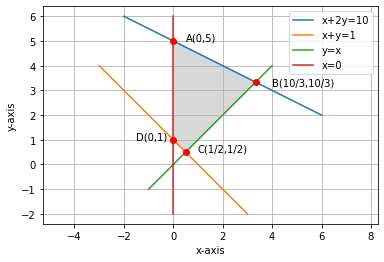
\includegraphics[width=\columnwidth]{solutions/su2021/2/58/Figures/Figure_2.58.png}
\caption{Graphical Solution}
\label{ineq/58/fig:fig1}	
\end{figure}

\begin{figure}[!ht]
\centering
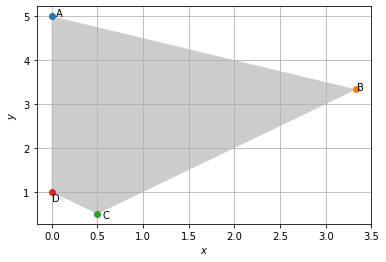
\includegraphics[width=\columnwidth]{solutions/su2021/2/58/Figures/2.58(2).png}
\caption{Magnified Solution region}
\label{ineq/58/fig:fig2}	
\end{figure}


    \item 2x-y $>$ 1, x-2y $<$ -1.
    \\
    \solution
    
%
Let
\begin{align}
\label{eq:1}
\begin{split}
2x-y &> 1,
\\-x+2y &> 1.
\end{split}
\end{align}
\\
Let $u_1 > 0, u_2 > 0$. This may be expressed as
\begin{align}
\vec{u} = \myvec{u_1\\u_2} &> \vec{0}
\end{align}
Now we have,
\begin{align}
\myvec{2&-1 \\ -1&2 }\vec{x} &> \myvec{1 \\ 1}   
\\
\myvec{2&-1 \\ -1&2 }\vec{x}-\vec{u} &= \myvec{1 \\ 1} 
\\
\text{or, } \myvec{2&-1 \\ -1&2 }\vec{x} &= \myvec{1 \\ 1}  + \vec{u}
\end{align}
Resulting in
\begin{align}
\vec{x} &= \myvec{2 & -1 \\ -1 & 2}^{-1}\myvec{1 \\ 1} +\myvec{2 & -1 \\ -1 & 2}^{-1} \vec{u}
\\
\vec{x }&=\myvec{1 \\ 1} +\frac{1}{3}\myvec{2 & 1 \\ 1 & 2}\vec{u}
\end{align} 
Thus , the solution of the system of inequalities can be determined graphically and the desired region is the shaded triangle which is represented in Fig. \ref{fig: Graphical Solution}
\begin{figure}[!ht]
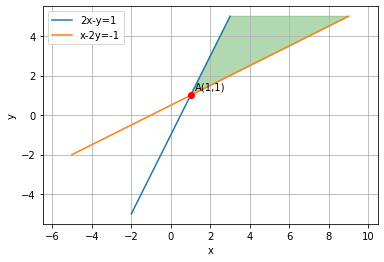
\includegraphics[width=\columnwidth]{solutions/su2021/2/50/Graphical Solution.png}
\caption{Graphical Solution}
\label{fig: Graphical Solution}
\end{figure}



    We obtain the vertices of the rhombus as follows
\begin{align}
\vec{A} = \myvec{-3\\0},
\vec{B} = \myvec{0\\-3.5},
\vec{C} = \myvec{3\\0},
\vec{D} = \myvec{0\\3.5}
\end{align}
which are plotted in Fig. \ref{quad/45/fig:Rhombus ABCD}.
%
\begin{figure}[ht!]
\centering
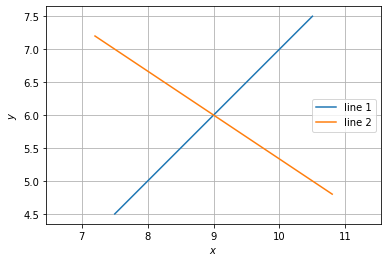
\includegraphics[width=\columnwidth]{solutions/quad/45/figure2.png}
\caption{Rhombus ABCD}
\label{quad/45/fig:Rhombus ABCD}
\end{figure}

    \item 2x+y $\geq$ 8, x+2y $\geq$ 10.
    \\
    \solution
    We obtain the vertices of the rhombus as follows
\begin{align}
\vec{A} = \myvec{-3\\0},
\vec{B} = \myvec{0\\-3.5},
\vec{C} = \myvec{3\\0},
\vec{D} = \myvec{0\\3.5}
\end{align}
which are plotted in Fig. \ref{quad/45/fig:Rhombus ABCD}.
%
\begin{figure}[ht!]
\centering
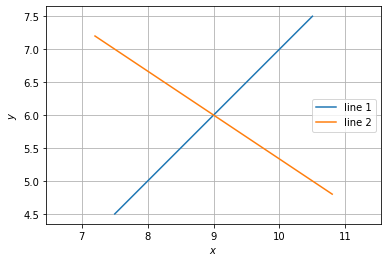
\includegraphics[width=\columnwidth]{solutions/quad/45/figure2.png}
\caption{Rhombus ABCD}
\label{quad/45/fig:Rhombus ABCD}
\end{figure}

    \item 3x+4y $\leq$ 60, x+3y $\leq$ 30, x $\geq$ 0, y $\geq$ 0.
    \\
    \solution
    
From the given inequalities we have,
\begin{align}
    \myvec{-3&-4 \\ -1&-3 \\ 1&0 \\ 0&1}\vec{x} \succeq \myvec{-60 \\ -30 \\ 0 \\ 0}
\end{align}
Which can be further written as
\begin{align}
   \myvec{-3&-4 \\ -1&-3 }\vec{x} \succeq \myvec{-60 \\ -30} 
\end{align}
Let $u_1 \ge 0, u_2 \ge 0$.  This may be expressed as
\begin{align}
\vec{u} = \myvec{u_1\\u_2}\succeq \vec{0}
\end{align}
Now we have,
\begin{align}
  \myvec{-3&-4 \\ -1&-3 }\vec{x} \succeq \myvec{-60 \\ -30}  + \vec{u} 
\end{align}
\begin{align}
        \vec{x} = \myvec{-3 & -4 \\ -1 & -3}^{-1}\myvec{-60 \\ -30} + \myvec{-3 & -4 \\ -1 & -3}^{-1}\vec{u}
        \\
        \implies \vec{x} = \frac{1}{5}\myvec{60 \\ 30}+\frac{1}{5}\myvec{-3&4 \\ 1&-3}\vec{u}
        \\
        \vec{x}=\myvec{12 \\ 6}+\frac{1}{5}\myvec{-3&4 \\ 1&-3}\vec{u}
    \end{align}
Thus the solution of the system of inequalities can be determined graphically, which is represented in Fig.     \ref{ineq/2/55/Graphical solution}.
%
\begin{figure}[ht]
    \centering
    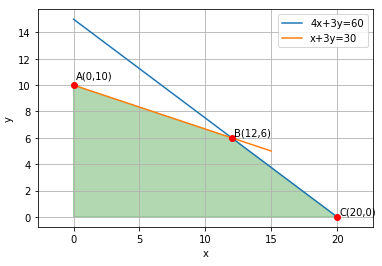
\includegraphics[width=\columnwidth]{solutions/su2021/2/55/Graphical solution region.PNG}
    \caption{Graphical solution}
    \label{ineq/2/55/Graphical solution}
\end{figure}






    \item x-2y $\leq$ 3, 3x+4y $\geq$ 12, x $\geq$ 0, y $\geq$ 1.
    \\
    \solution
    


\begin{figure}[!ht]
    \centering
    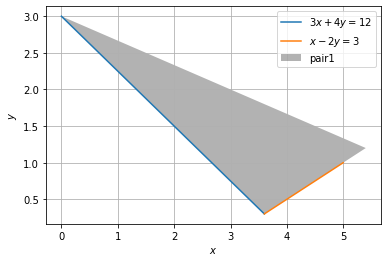
\includegraphics[width=\columnwidth]{solutions/su2021/2/56/Figure9_1.png}
    \caption{Inequality pair 1}
    \label{ineq/56/fig:inequalities1}	
    \end{figure}
    
    \begin{figure}[!ht]
    \centering
    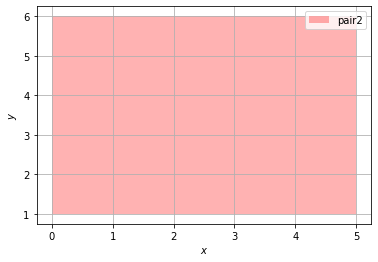
\includegraphics[width=\columnwidth]{solutions/su2021/2/56/Figure9_2.png}
    \caption{Inequality pair 2}
    \label{ineq/56/fig:inequalities2}	
    \end{figure}
    
    \begin{figure}[!ht]
    \centering
    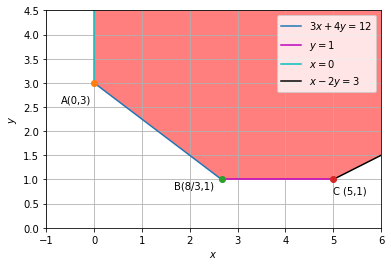
\includegraphics[width=\columnwidth]{solutions/su2021/2/56/Figure 9_3.png}
    \caption{Intersection of \ref{ineq/56/fig:inequalities1} and \ref{ineq/56/fig:inequalities2}}
    \label{ineq/56/fig:inequality3}	
    \end{figure}
    The common region shown by \ref{ineq/56/fig:inequality3} is the solution of set of inequalities.
    
    \item 4x+3y $\leq$ 60, y $\geq$ 2x, x $\geq$ 3, x,y $\geq$ 0.
    \\
    \solution
    

The given system of inequality can be written in matrix form as
\begin{align}
    \myvec{-4 & -3 \\ -2 & 1 \\ 1 & 0 \\ 1 & 0 \\ 0 & 1}\vec{x} \succeq \myvec{-60\\0\\3\\0\\0}
\end{align}
which can be further simplified into 
\begin{align}
    \myvec{-4 & -3 \\ 1 & 0 \\ 0 & 1}\vec{x} \succeq \myvec{-60\\3\\6}
\end{align}

Let the surplus vector be
\begin{align}
    \vec{u} &= \myvec{u_1\\u_2} \succeq 0
\end{align}

\begin{enumerate}
    \item 
    \begin{align}
        \myvec{-4 & -3 \\ 1 & 0}\vec{x} &\succeq \myvec{-60 \\ 3}
        \\
        \implies  \myvec{-4 & -3 \\ 1 & 0}\vec{x} &= \myvec{-60 \\ 3} + \vec{u}
    \end{align}
    resulting in 
    \begin{align}
        \vec{x} &= \myvec{-4 & -3 \\1 & 0}^{-1}\myvec{-60 \\ 3} + \myvec{-4 & -3 \\1 & 0}^{-1}\vec{u}
        \\
        \implies \vec{x} &= \myvec{3 \\16} + \myvec{0 & 1\\ \frac{-1}{3} & \frac{-4}{3}}\vec{u}   \label{ineq/2/57eq1}
    \end{align}

    \item 
    \begin{align}
        \myvec{-4 & -3 \\ 0 & 1}\vec{x} &\succeq \myvec{-60 \\ 6}
        \\
        \implies  \myvec{-4 & -3 \\ 0 & 1}\vec{x} &= \myvec{-60 \\ 6} + \vec{u}
    \end{align}
    resulting in 
    \begin{align}
        \vec{x} &= \myvec{-4 & -3 \\0 & 1}^{-1}\myvec{-60 \\ 6} + \myvec{-4 & -3 \\0 & 1}^{-1}\vec{u}
        \\
        \implies \vec{x} &= \myvec{\frac{21}{2} \\6} + \myvec{\frac{-1}{4} & \frac{-3}{4}\\ 0 & 1}\vec{u} \label{ineq/2/57eq2}
    \end{align}
\end{enumerate}

Now,solution region which is common to regions of eq. \eqref{ineq/2/57eq1} and eq. \eqref{ineq/2/57eq2},is given by

\begin{align}
    \boxed{\vec{x} = \myvec{3 \\ 6}+\myvec{0 & 1\\\frac{1}{12} & \frac{-13}{12}}\vec{u}}
\end{align}


\begin{figure}[!ht]
\centering
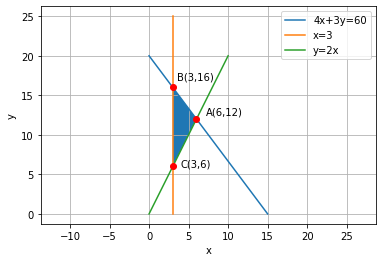
\includegraphics[width=\columnwidth]{solutions/su2021/2/57/Figures/Figure11_1.png}
\caption{Solution Region}
\label{ineq/2/57fig:fig1}	
\end{figure}

% \numberwithin{figure}{section}
% \begin{figure}[!ht]
% \centering
% 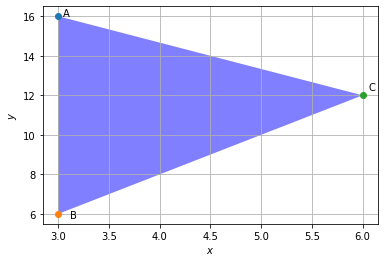
\includegraphics[width=\columnwidth]{Figure11_2}
% \caption{Magnified Solution Region}
% \label{ineq/2/57fig:fig2}	
% \end{figure}




%\end{document}

